\documentclass[9pt,twocolumn,twoside]{../../styles/osajnl}
\usepackage{fancyvrb}
\journal{i524} 

\title{Berkeley DB}

\author[1,*]{Saber Sheybani}

\affil[1]{School of Informatics and Computing, Bloomington, IN 47408, U.S.A.}

\affil[*]{Corresponding authors: sheybani@indiana.edu}

\dates{Paper 2, \today}

\ociscodes{NoSQL, embedded database, Oracle, open source database management system}

\doi{\url{https://github.com/cloudmesh/sp17-i524/tree/master/paper2/S17-ER-1001/report.pdf}}



\begin{abstract}
Berkeley DB is a family of open source, NoSQL key-value database libraries. It provides a simple function-call API for data access and management over a number of programming languages, including C, C++, Java, Perl, Tcl, Python, and PHP. Berkeley DB is embedded because it links directly into the application and runs in the same address space as the application. As a result, no inter-process communication, either over the network or between processes on the same machine, is required for database operations. It is also extremely portable and scalable, it can manage databases up to 256 terabytes in size.
For data management, Berkeley DB offers advanced services, such as concurrency for many users, ACID transactions, and recovery. 
Berkeley DB is used in a wide variety of products and a large number of projects, including gateways from Cisco, Web applications at Amazon.com and open-source projects such as Apache and Linux.
\newline
\end{abstract}

\setboolean{displaycopyright}{true}

\begin{document}

\maketitle

\section{Introduction}

Data management has always been a fundamental issue in programming.
Since 1960s, countless database management systems have been developed 
to fulfil different sorts of demands. The question for every user is choosing the 
system that best fits the requirements of its appliction.

Database management systems can be categorized based on data models, into a 
number of groups: Hierarchical Databases, Network Databases, Relational Databases, Object-based Databases, and Semistructured Databases.
\newline 
\textbf{Hierarchical} databases use the oldest type of data models, which is a tree-like structure. 
The records are connected to each other with a hard-coded link.
\newline 
In a \textbf{Network} model, records are also connected with links, but there is no hierarchy. Instead, the structure is graph-like
and all of the nodes can connect to each other.
\newline 
In \textbf{Relational} databases, there are no physical links, but the data is structured 
in tables (relations). Each row represents a record and each column represents an attribute. 
The tables are connected with common attributes, which makes querying
much easier than the two former models. For this reason, database management systems
using relational models are the most widely used ones.
\newline 
\textbf{Object-based} data models extend concepts of object-oriented programming into database systems, 
in order to provide persistent storage of objects and other capabilities of databases
for object-oriented programming.
\newline
\textbf{Semistructured} databases which include NoSQL databases are the type of database model
that enable storage of hetereogenous data, by allowing records with different attributes.
This however, is achieved by sacrificing the knowledge of data type by the database system.
The data in this case must be \textit{self-describing}, meaning that the description (schema) of the
data must be in itself. XML (Extensible Markup Language) schema language is a widely used language
for providing schema for these database systems\cite{limited2010introduction}.  

Berkeley DB fits into the last category, as a NoSQL database system. The records are stored 
as key-value pairs and a few logical operations can be executed on them, namely:
insertion, deletion, finding a record by its key, and updating an already found record. 
"Berkeley DB never operates on the value part of a record. Values are simply payload, 
to be stored with keys and reliably delivered back to the application on demand." 
There is no notion of schema and no support for SQL queries. "The application must 
understand the keys and values that it uses. On the other hand, there is literally 
no limit to the data types that can be stored in a Berkeley DB database. The application 
never needs to convert its own program data into the data types that Berkeley DB supports. 
Berkeley DB is able to operate on any data type the application uses, no matter how complex"
\cite{stanford-dbisnot}.

\section{Architecture}

Berkeley DB's architecture can be explained by five major subsystems: 
\textbf{Access Methods}: Providing general-purpose support for creating and accessing database files.
\textbf{Memory Pool}: The general-purpose shared memory buffer pool. Multiple 
\textbf{Transaction}: Implementing the transaction model, realizing ACID properties.
processes and threads within processes share access to databases using this subsystem.
\textbf{Locking}: The general-purpose lock manager for processes.
\textbf{Logging}: The write-ahead logging that supports the Berkeley DB transaction model.

\begin{figure}[htbp]
\centering
\fbox{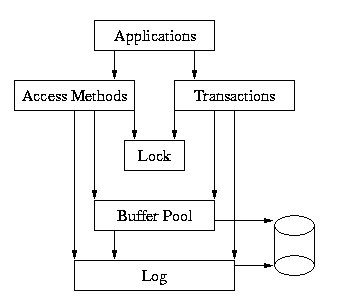
\includegraphics[width=\linewidth]{images/BDB_Subsystems_Diagram.png}}
\caption{Berkeley DB Subsystems \cite{stanford-bigpic}}
\label{fig:subsystems}
\end{figure}

Figure \ref{fig:subsystems} displays a diagram of the Berkeley DB library architecture. 
The arrows are calls that invoke the destination. Each subsystem can also be used 
independent from the other ones, but this usage is not common.


\section{Services and Other Features}

The two fundamental services that every database management system provides are data access, 
and data management services. Data access services include the low-level operations on the 
records, which were already mentioned in the introduction for the case of Berkeley DB.
In terms of storage structure, Berkeley DB supports \textbf{hash tables, Btrees, simple 
record-number-based storage, and persistent queues} \cite{stanford-dbis}.

Data management services are the higher-level services (and features) such as concurrency that 
ensure specific qualities for operation of the system. These services include allowing simultaneous
access to the records by multiple users (concurrency), changing multiple records at the same 
time (transaction), and complete recovery of the data from crashes (recovery) \cite{stanford-dbis}. 
\newline
For \textbf{concurrency}, Berkeley DB is able to handle low-level services such as locking and 
shared buffer management transparently, while multiple processes and threads use the data.
\newline 
For recovery, every application can ask Berkeley DB for recovery, at startup time.
\newline
An \textbf{ACID transaction} ensures the following specifications at the end of its operation 
\cite{haerder1983principles}: Atomicity (Either all or none of the records change), Consistency 
(The system goes from one valid state to another), Isolation (concurrent execution of multiple 
transaction yields the same result as the sequential execution of them), Durability (The result 
remains steady, even in case of crash of the system).Berkeley DB "libraries provide strict ACID 
transaction semantics, by default. However, applications are allowed to relax the isolation 
guarantees the database system makes" \cite{stanford-dbis}.

Berkeley DB runs in the same address space as the application. As a result, there is no need 
for communication between processes and threads. On the other hand, as an embedded 
database management system, it does not provide a standalone server. However, server 
applications can be built over Berkeley DB and many examples of Lightweight Directory Access 
Protocol (LDAP) servers have been built using it \cite{stanford-dbisnot}.

The database library for Berkeley DB consumes less than 300 kilobytes of text space on common 
architectures. That makes it a feasible solution for embedded systems with small capacities.
Nonetheless, it can manage up to 256 terabytes databases. 

\subsection{Supported Operating Systems and Languages}

Berkeley DB supports nearly all modern operating systems. They include Windows, Linux, Mac OS X,
Android, iPhone, Solaris, BSD, HP-UX, AIX, and RTOS such as VxWorks,and QNX.
\newline
The supported programming languages include "C, C++, Java, C\#, Perl, Python, PHP, Tcl, Ruby and 
many others" \cite{bdb-datasheet}.

\subsection{Required Infrastructure}
As infrastructure, Berkeley DB requires "underlying IEEE/ANSI Std 1003.1 (POSIX) system calls and 
can be ported easily to new architectures by adding stub routines to connect the native system 
interfaces to the Berkeley DB POSIX-style system calls" \cite{stanford-web}.

\section{Products and Licensing}

The products include three implementations on C, C++, and Java (Oracle Berkeley DB, Oracle Berkeley 
XML, and Oracle Berkeley JE, respectively) \cite{oracle-products}.
\newline
Berkeley DB is an open source library and is free for use and redistribution in other open source products. 
the distribution includes complete source code for all three implementations, their supporting utilities, 
as well as complete documentation in HTML format \cite{stanford-web}.

For redistribution in commercial products, Sleepycat Software licenses four products, with prices 
ranging from US\$900 to 13,800 per processor \cite{oracle-price} as of March 2017. The products, 
in the order of ascending price and capabilities are: Berkeley DB Data Store, Berkeley DB Concurrent Data Store,
Berkeley DB Transactional Data Store, Berkeley DB High Availability.
The Sleepycat software also includes prebuilt libraries and binaries as part of support services, which is not provided in the free distribution.
There is no additional license payment for embedded usage within the Oracle Retail Predictive Application Server (RPAS).

\section{Use Cases}
A notable number of open source and commercial products in different areas of technology, use Berkeley DB. 
Open source use cases include Linux, UNIX, BSD, Apache, Solaris, MySQL, Sendmail, OpenLDAP, and MemcacheDB.
\newline 
Proprietary applications "include directory servers from Sun and
Hitachi; messaging servers from Openwave and LogicaCMG; switches, routers and
gateways from Cisco, Motorola, Lucent, and Alcatel; storage products from EMC and
HP; security products from RSA Security and Symantec; and Web applications at
Amazon.com, LinkedIn and AOL" \cite{bdb-datasheet}.

\section{Advantages and Limitations}

Berkeley DB has two advantages over relational and object-oriented database systems, when it comes to embedded applications.
One is running in the same address space as the application and thus, not requiring any inter-process communication which 
can have a high cost in embedded applications. And the other is simplicity of interface for operations which does not require 
query language parsing. These two features along with its small size, give Berkeley DB system a privilege of being lightweight
enough for many applications where there are tight constraints on resources.
\newline
However, with simplicity comes the lack of SQL features. If the user of the application 
needs to perform complicated searches (potentially using SQL queries) the programmer would 
need to write the code for those cases. In general, Berkeley DB is aimed at providing fast, 
reliable, transaction-protected record storage, at a minimalist way \cite{stanford-need}.

\section{Educational Material}

As was mentioned in the Products section, the free distribution comes with complete 
documentation in HTML format. The documentation has two parts: a reference manual in UNIX-style for programmers,
and a reference guide which can serve as a tutorial \cite{olson1999berkeley}.
In addition to that, \emph{Berkeley DB Tutorial and Reference Guide, Version 4.1.24} 
\cite{stanford-web} and \emph{The Berkeley DB Book} \cite{yadava2007berkeley} are useful 
resources for learning more about Berkeley DB and getting started with it.

\section{Conclusion}

Berkeley DB is a minimal, lightweight database management system, focused on providing 
performance, especially in embedded systems. It offers a small, simple set of data access 
services, and  a rich powerful set of data management services. It is freely available 
for use by non-commercial distributions and has been successfully used in many projects.

% Bibliography

\bibliography{references}
 
\section*{Author Biography}
\begingroup
\setlength\intextsep{0pt}
\begin{minipage}[t][3.2cm][t]{1.0\columnwidth} % Adjust height [3.2cm] as required for separation of bio photos.
  \noindent
  {\bfseries Saber Sheybani} received his B.S. (Electrical Engineering - Minor in Control Engineering) from University of Tehran.  He is currently a PhD student of Intelligent Systems Engineering - Neuroengineering at Indiana University Bloomington.
\end{minipage}
\endgroup

\end{document}
